\section{Red a analizar}

De cara a realizar esta práctica se va a analizar la red de seguidores de la Escuela Técnica Superior de Ingenierías Informática y de Telecomunicación (ETSIIT), de la Universidad de Granada.

He escogido esta red ya que me parece interesante estudiar las conexiones que puede tener la ETSIIT al ser un centro donde coinciden distintos perfiles, investigadores, estudiantes, docentes, empresas, instituciones, etc, lo que puede ser interesante ver y comprender como interactúan todo este tipo de perfiles, y observar si es fácil hacer estas distinciones entre perfiles.

\subsection{Obtención de los datos de la red}

Para obtener los datos de los seguidores de Twitter he utilizado la herramienta twitter-graph \cite{twitterGraph}. Esta herramienta permite utilizar nuestras credenciales de desarrollador de Twitter para realizar peticiones a la API de Twitter, como obtener los seguidores y conexiones de cierto usuario, buscar por términos concretos en todo Twitter, o obtener los me gusta a los que le ha dado un usuario.

En nuestro caso se ha utilizado para obtener los datos de los seguidores de la cuenta de la ETSIIT \cite{twitterETSIIT}. Al utilizar esta herramienta se nos ha generado dos ficheros csv, uno con los datos de los nodos y otro con la información de los enlaces.

\subsection{Previsualización de toda la red}

Una vez exportamos los datos a Gephi, podemos visualizar la red. De cara a poder visualizarla sin perder resolución, se ha exportado como PDF y se ha incrustado la página obtenida en esta memoria. Se ha utilizado el algoritmo ForceAtlas 2 para visualización, intentando que la red quede lo más estética posible, pero como vamos a ver se trata de una red muy densa, donde existen muchas conexiones y no es sencillo hacer un primer análisis visual claro.

Esta visualización es la generada directamente por Gephi, por lo que podemos hacer zoom a dicha visualización para poder ver en detalle la red.

\newpage
\begin{figure}[H]
	\centering
	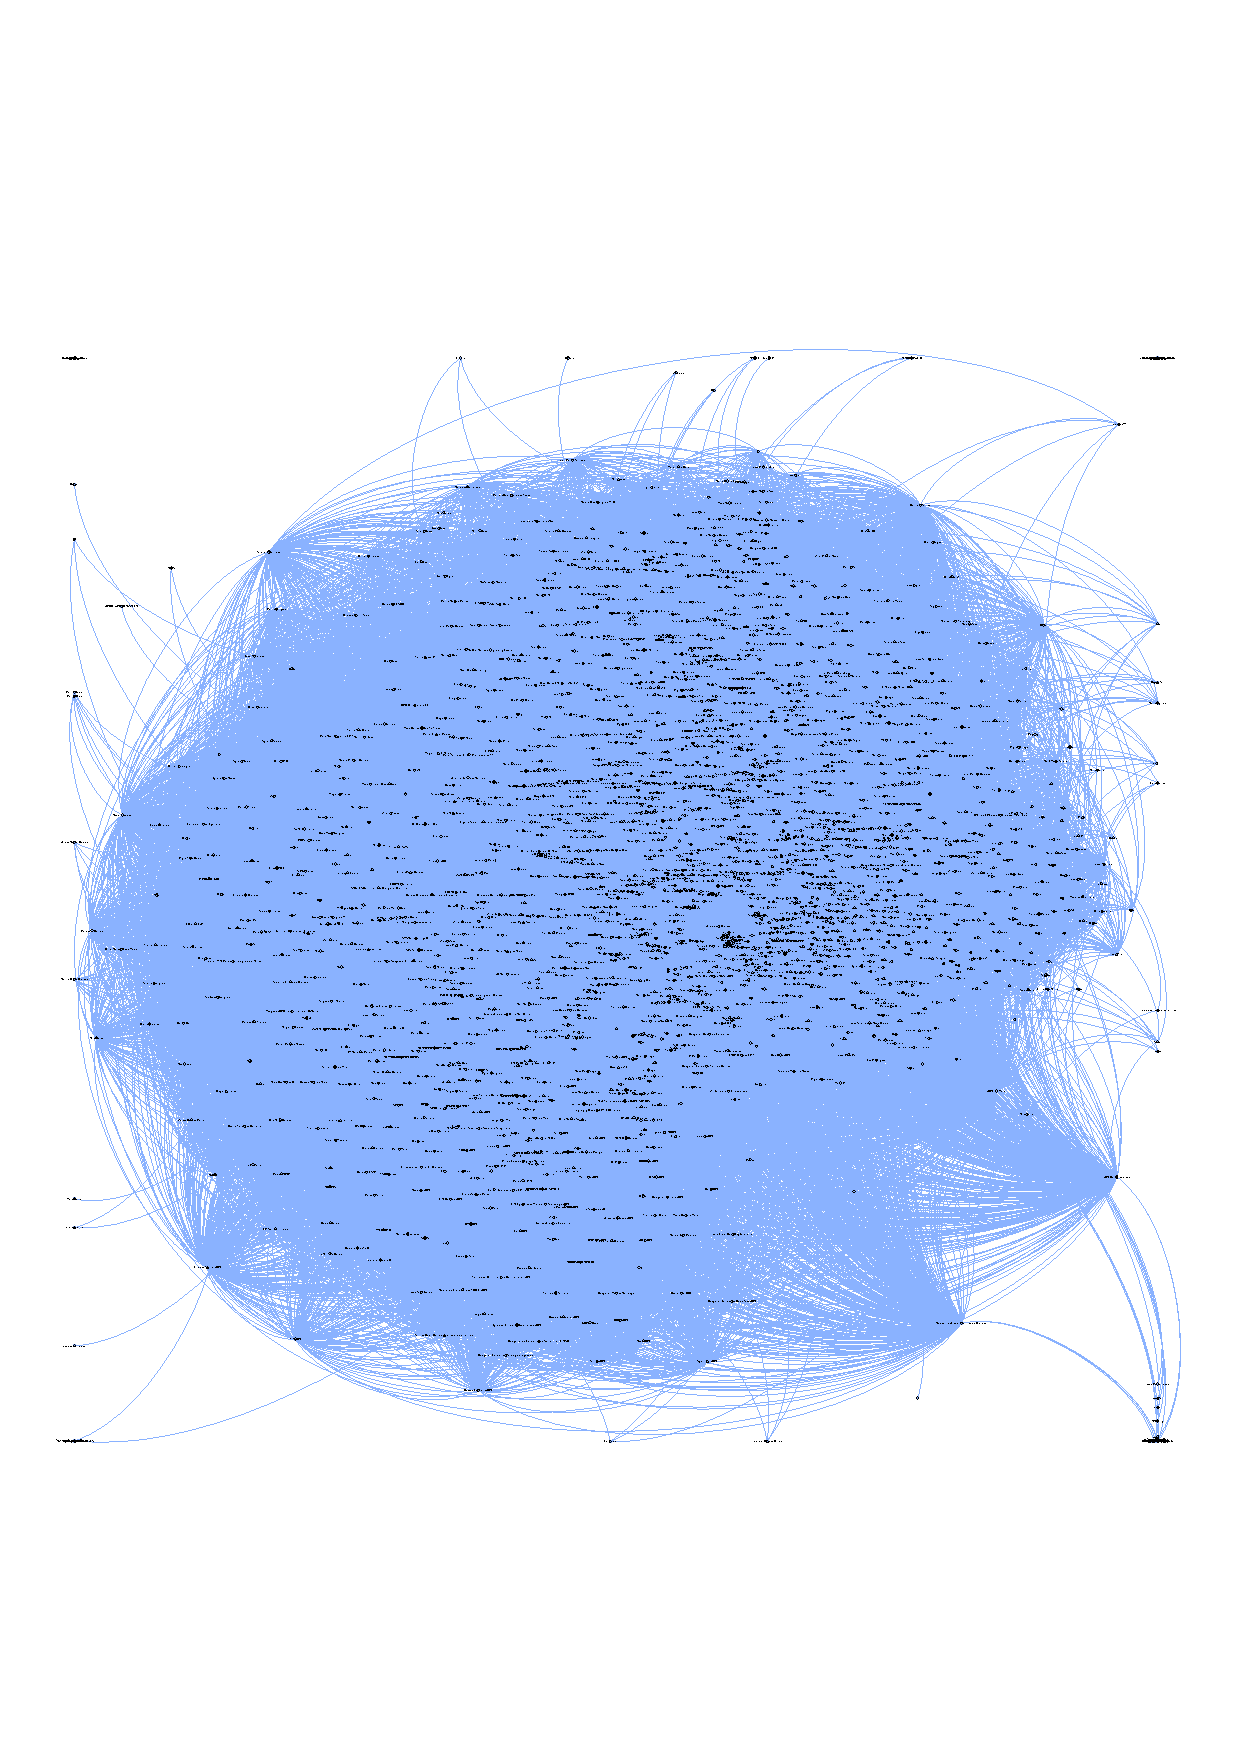
\includepdf[frame=true, scale=0.9, offset=75 -50]{pdf_incrustados/red_completa.pdf}
	\caption{Red completa de seguidores de la cuenta ETSIIT}
\end{figure}
\newpage


\subsection{Previsualización de la componente gigante de la red}

\subsection{Medidas de la red}

\subsection{Gráficos sobre las medidas de la red}
